% !TEX root = ../main.tex

\section{Introduction}
\label{sect:introduction}

Ethereum blockchain project~\cite{EthGit} was launched in 2014 by announcing Ether as its protocol-level cryptocurrency\footnote{A digital currency in which encryption techniques are used to regulate the generation of units of currency and verify the transfer of funds, operating independently of a central bank.}. According to \textit{CoinMarketCap}, which ranks cryptocurrencies that are actively traded on an exchange service, Ether is ranked second after Bitcoin\footnote{CoinMarketCap-Ethereum currency - [2019-07-11] \url{https://coinmarketcap.com/currencies/ethereum/}} in 2019. It also has the biggest development community to track enhancement and introduce new ideas\footnote{CoinDesk Crypto-Economics Explorer - [2019-07-11] \url{https://www.coindesk.com/data}}. Ethereum allows users to build decentralized applications (DApps) in the form of smart contracts; computer programs that are written in a high-level programming language called Solidity~\cite{Solidity7:online}. Migrating applications from centralized to decentralized architecture can solve many issues (\textit{e.g.,} single point of failure, hardware and maintenance costs, data security, distributed trust, \textit{etc.}). Distributed property of the blockchain removes single point of failure (SPOF) and increases resiliency of the deployed applications on top of it. If one node faced hardware or communication failures, other nodes would continue responding to the coming requests since they have full copy of data locally.

DApps can accept and use Ethereum’s protocol-level currency (Ether) or issue their own custom currency-like tokens. Tokens are standardized version of smart contracts\footnote{Can be considered as smart transaction: Types of transactions that execute as they are programmed by a scripting language (like Solidity or Viper). Logic of the transaction is dynamic and can represent an application.} that define common set of rules (known as API\footnote{Advanced Programming Interface.}). The Ethereum project accepted a proposed standard called ERC20-- the most popular token standard on the Ethereum. It is in fact an interface defines 6 abstract methods and 2 events (see Figure~\ref{fig:erc20api}). Having a token standard provides interoperability with other applications (\textit{e.g.,} wallets, decentralized application, web services, \textit{etc.}). Other applications would be aware of functionalities of tokens and available methods to use. ERC20 standard does not provide an actual concrete implementation and only provides guidelines on how each method should be implemented (such as name of the method, parameters, return types). This gives developers flexibility of coding based of requirements of their DApps. The point here is that all ERC20-compliant tokens must implement these 6 methods and 2 events. They are not optional and this constraint makes ERC20 tokens interoperable with other DApps or web services. In other words, other applications would be aware of how to communicate with ERC20 tokens. 

\begin{figure}[t]
	\centering
	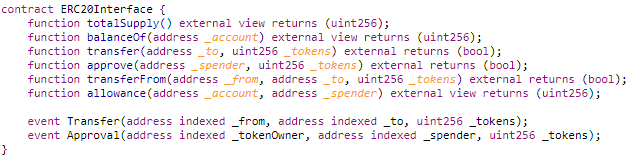
\includegraphics[width=0.8\linewidth]{figures/img02.png}
	\caption{An interface declaring the required functions and events to meet the ERC20 standard.}
	\label{fig:erc20api}
\end{figure}

A use case of Ethereum tokens could be considered when implementing a decentralized trading system (see Figure~\ref{fig:erc20ex}). Since the application will be running on the blockchain, we need to represent corresponding financial assets as tokens. Leveraging ERC20 tokens facilitate implementation of left side of this trading model (which is share of company X). Correspondingly, the right side needs a financial asset which is equivalent to a fiat currency (like USD or CAD). Stablecoins\footnote{Types of digital assets that value of it will be stable over time and people be able to count on its value since it is pegging to something that has a stable value (like gold or USD).} provide this functionalities and could also be represented as ERC20 token.

\begin{figure}[t]
	\centering
	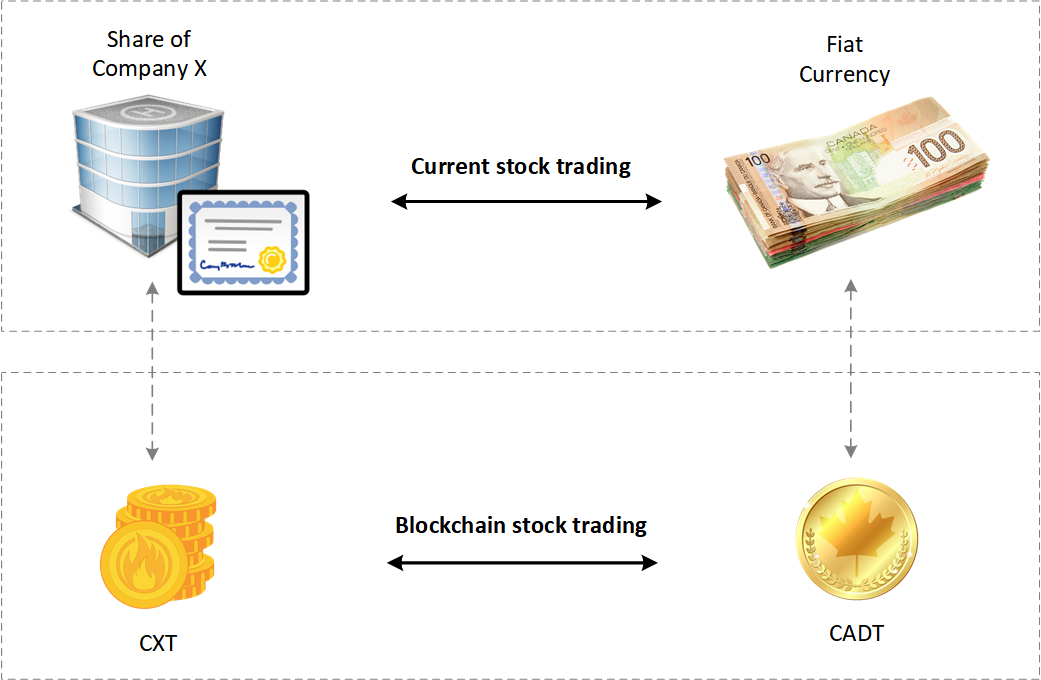
\includegraphics[width=0.78\linewidth]{figures/img01.png}
	\caption{A blockchain trading model using ERC20 tokens to leverage blockchain as a distributed platform. ERC20 standard makes it possible to migrate financial assets to their digital representation on the blockchain.}
	\label{fig:erc20ex}
\end{figure}

Representing both financial assets as ERC20 tokens, gives us two ERC20 tokens with different values to trade. This shows the importance of tokens in Ethereum ecosystem for digitizing tangible assets to digital equivalents on the blockchain. By using ERC20 tokens, we are able to migrate current centralized trading systems to decentralized equivalent and taking advantage of a distributed trading system on the blockchain. Being subset of smart contracts make ERC20 tokens vulnerable to security threats. In this report, we analyze major identified ERC20 vulnerabilities and discuss their mitigations. By considering them in a reference implementation, we would be able to propose a secure version of ERC20 token that addresses these security issues and can be used for deployment of secure tokens on the Ethereum blockchain.

\section{Motivation}
The development of smart contracts has proven to be error-prone in practice, and as a result, smart contracts deployed on public platforms are often riddled with security vulnerabilities -- previous research~\cite{MakSm} showed that at about 45\% of existing smart contracts are vulnerable to security threads. Similar to any other smart contract, ERC20 token are also vulnerable to security flaws. There are currently at about 205,787\footnote{https://etherscan.io/tokens, Accessed 12-Aug-2019} ERC20 tokens on the Ethereum blockchain\footnote{64,000 functional ERC20 tokens as of early 2019~\cite{victormeasuring}} that might be vulnerable to one of these issues.  To address this concern, we focus on identified ERC20 vulnerabilities (such as overflow issue, multiple withdrawal, re-entrancy attack, \textit{etc.}) and research on recommended mitigations. By putting all these solutions together, we will be able to propose a secure implementation of ERC20 token that can be used as a reference model for future ERC20 implementations. Developers can also refer to each mitigation separately to address a specific attack in their migrated ERC20 tokens.

In addition to increasing security of ERC20 tokens, some tokens have considerable value that potentially exceeding the value of Ether itself (\textit{e.g.,} MKR\footnote{\url{https://makerdao.com/en/}, [Accessed online: July 27, 2019]} at \$580 and XIN\footnote{\url{https://mixin.one/}, [Accessed online: July 27, 2019]} at \$210). Similar to other financial assets, ERC20 tokens might be audited. Existence of security thread will impact ownership of tokens that may lead to hesitation of auditors. Therefore, providing attack severity helps auditors to better assess associated risk of ERC20 tokens.

\section{Contributions}
This paper provides an overview of three major vulnerabilities (overflow attack, multiple withdrawal attack, and re-entrancy attack) on Ethereum's most popular token standard; Ethereum ERC20 tokens. We carefully select these vulnerabilities based on their attack vector and broader impact on the Ethereum blockchain. For each of the selected vulnerabilities, we (i) thoroughly \textbf{explain} and \textbf{visualize} the technical details , (ii) reproduce the attack using \textit{Solidity} programming language (attack demo), (iii) provide the severity and technical details of how to mitigate and/or prevent the attack. Eventually, we \textbf{propose} a secure ERC20 standard for the Ethereum blockchain that is not vulnerable to any of the vulnerabilities discussed. We ultimately implement, deploy, and test our ERC20 proposal on Rinkeby\footnote{Similar to the Ethereum main net but it is designed for testing contracts. Ethers are not real on it and it is just for testing. It can be requested via \url{https://faucet.rinkeby.io}}. The proof of concept of our proposal can be found in Section~\ref{sec:proposal}.

